\documentclass[12pt,a4paper]{article}
\emergencystretch=3cm

\usepackage[margin=1in]{geometry}
\usepackage{graphicx}
\usepackage{setspace}
\usepackage{times}
\usepackage{titlesec}
\usepackage{amsmath, amssymb, amsthm}
\usepackage{booktabs}
\usepackage{array}
\usepackage{hyperref}
\usepackage{enumitem}
\usepackage{fancyhdr}
\usepackage{indentfirst}
\usepackage{float,caption,xcolor,microtype,listings}
\captionsetup{font=small,labelfont=bf}
\lstset{basicstyle=\ttfamily\scriptsize,backgroundcolor=\color{black!5},frame=single,rulecolor=\color{black!40},breaklines=true,columns=fullflexible,keepspaces=true,aboveskip=0.6em,belowskip=0.4em}
\graphicspath{{../figures/}}
\newcommand{\code}[1]{\texttt{\small #1}}

\hypersetup{
    colorlinks=true,
    linkcolor=black,
    citecolor=black,
    urlcolor=blue
}

\onehalfspacing
\setlength{\parindent}{0.5in}
\setlength{\parskip}{0pt}

\titleformat{\section}
    {\normalfont\bfseries\large}{\thesection.}{0.5em}{}
\titleformat{\subsection}
    {\normalfont\bfseries}{\thesubsection.}{0.5em}{}

\pagestyle{fancy}
\fancyhf{}
\setlength{\headheight}{14.5pt}
\fancyhead[L]{\small Model Comparison for Heart Disease Prediction}
\fancyhead[R]{\thepage}
\renewcommand{\headrulewidth}{0.4pt}


\begin{document}

\begin{titlepage}
    \centering

    \begin{minipage}[c]{0.20\textwidth}
        \centering
        
\includegraphics[height=1.1in,keepaspectratio]{assets/bulsu.png}
    \end{minipage}%
    \begin{minipage}[c]{0.56\textwidth}
        \centering
        {\Large\bfseries Bulacan State University\par}
        \vspace{0.15cm}
        {\large\bfseries College of Science\par}
        \vspace{0.15cm}
        {\normalsize MCS 306: Introduction to AI\par}
        \vspace{0.15cm}
        {\normalsize Academic Year 2026--2027\par}
    \end{minipage}%
    \begin{minipage}[c]{0.20\textwidth}
        \centering
        
\includegraphics[height=1.1in,keepaspectratio]{assets/college_of_science.png}
    \end{minipage}

    \vfill

    {\Large\bfseries MINI RESEARCH AND EXPOSITION PAPER\par}

    \vspace{0.4in}

    {\Large\bfseries Comparing Logistic Regression, Decision Tree, and K-Nearest Neighbors Against a Majority-Class Baseline for Heart Disease Prediction\par}

    \vfill

    {\large\bfseries Authors\par}
    \vspace{0.2cm}
    {\large Bon Federique B. Avendano,\\ Leonicos Chael C. De Robles,\\ Clarence Wayne B. Ignacio,\\ Jerol Liuz V. Manlapig,\\ Brylle James G. Robles\par}

    \vspace{0.3in}

    {\large BSM CS-3B\par}

    \vfill

    {\normalsize Submitted to:\par}
    \vspace{0.15cm}
    {\normalsize\bfseries Aarhus M. Dela Cruz\par}

    \vspace{0.3in}

    {\normalsize October 31, 2026\par}
\end{titlepage}

\pagenumbering{roman}
\setcounter{page}{1}

\begin{abstract}\noindent
Cardiovascular disease is the leading global cause of death, and routine clinical measurements could support early screening if they are turned into reliable risk estimates. This study compares three supervised classifiers---logistic regression, a decision tree, and K-nearest neighbors (KNN)---against a majority-class baseline on the Heart Failure Prediction Dataset (918 patients, 11 predictors, 55.3\% positive). All preprocessing (median imputation, scaling, one-hot encoding) is fitted inside scikit-learn pipelines to prevent leakage; hyperparameters are tuned by 5-fold cross-validation on a stratified 75\% training split; models are compared by nested cross-validation and then evaluated once on a 25\% held-out test set. The baseline, which predicts ``heart disease'' for everyone, reaches 55.2\% accuracy and an F1 of 0.712 but has zero specificity and an MCC of 0, showing that accuracy and F1 alone are misleading even in a mildly imbalanced problem. All three models beat the baseline decisively (McNemar $p<10^{-10}$). Logistic regression ($C=1$) and KNN ($k=21$) performed best and were statistically indistinguishable (test ROC AUC 0.933 and 0.939; accuracy 0.887 and 0.883), while the depth-5 decision tree was weaker (AUC 0.908; accuracy 0.843) but the most interpretable. Under an assumed 5:1 false-negative-to-false-positive cost, an out-of-fold threshold cut expected cost from 74--120 to 54--69 units, below the baseline's 103. We recommend logistic regression as the default screening model because it matches KNN's accuracy, is transparent, and needs no stored training set. Because the data pool five hospitals and the test set has only 230 patients, any deployment would first require local validation.
\end{abstract}

\noindent\textbf{Keywords:} heart disease, logistic regression, decision tree, K-nearest neighbors, majority baseline, nested cross-validation

\newpage
\tableofcontents
\newpage

\pagenumbering{arabic}
\setcounter{page}{1}

%================ 1 INTRODUCTION ================
\section{Introduction}
Cardiovascular disease (CVD) remains the leading cause of death worldwide; the World Health Organization (2025) reports that 19.8 million people died from it in a single year, about 32\% of all deaths. Heart failure, in which the heart cannot pump enough blood to meet the body's needs, is one of its most serious forms, and early detection is central to timely treatment. Diagnosis traditionally combines patient history, physical examination, electrocardiography, and laboratory tests, and the interpretation of these records can vary between practitioners. Machine-learning classifiers offer a complementary, data-driven option: given routinely recorded measurements, they output an estimated probability that a patient has heart disease, which can flag high-risk patients at first contact.

An earlier group report (Avendano et al., 2026) built a KNN screening pipeline for this problem. That raises a natural follow-up question that a single-model study cannot answer: \emph{is KNN actually the right model, and how much better than doing nothing is it?} A model's score only has meaning relative to alternatives. Two kinds of comparison are therefore needed: (i) against a \emph{trivial baseline}, which shows whether the data contain any learnable signal, and (ii) against \emph{other standard classifiers}, which shows whether the extra complexity of a method is justified.

\subsection{Research Question}
\noindent On the same patient records, how do logistic regression, a decision tree, and KNN compare with each other and with a majority-class baseline in accuracy, error structure, discrimination, interpretability, and computational cost?

\subsection{Objectives of the Paper}
The objectives of this paper are as follows:
\begin{enumerate}[label=\arabic*.,itemsep=0pt]
  \item Build a leakage-resistant workflow in which every data-dependent step is learned from training data only.
  \item Tune each model's key hyperparameter by cross-validation and compare the four models with nested cross-validation.
  \item Evaluate each model once on a held-out test set with accuracy, precision, recall, specificity, F1, balanced accuracy, MCC, ROC AUC and PR AUC, with uncertainty estimates and paired significance tests.
  \item Examine a cost-sensitive decision threshold and discuss interpretability, runtime, and limitations.
\end{enumerate}
\subsection{Significance and Relevance of the Models}
\noindent The three models represent three different ways of learning from data: a linear parametric model (logistic regression), a rule-based partitioning model (decision tree), and a non-parametric instance-based model (KNN). Together with the majority baseline they cover the usual spectrum from ``no learning'' to ``flexible learning'', making the comparison informative for a screening tool in which transparency matters as much as accuracy.

%================ 2 PRELIMINARIES ================
\section{Review of Related Literature and Background Concepts}
\subsection{Related Studies}
Heart-disease prediction has long been studied on the combined clinical collections that form this dataset; the original Cleveland, Hungarian, Switzerland and Long Beach VA data derive from a multinational study of coronary artery disease diagnosis (Detrano et al., 1989), and the merged file used here was published by Fedesoriano (2021). The group's earlier report (Avendano et al., 2026) applied KNN with SMOTE oversampling and a sensitivity-weighted threshold to the same records, but evaluated a single model without a reference point. The present paper complements it with a trivial baseline and two other standard classifiers, evaluated under a stricter leakage-resistant protocol. On the methodological side, we draw on work showing that tuned models should be compared by nested cross-validation (Varma \& Simon, 2006), that precision--recall and MCC summaries are more informative than accuracy under class imbalance (Saito \& Rehmsmeier, 2015; Chicco \& Jurman, 2020), that classifiers should be compared with paired tests on shared test cases (Dietterich, 1998), and that decision thresholds should reflect unequal error costs (Elkan, 2001).

\subsection{Key Definitions}
\subsubsection{Binary classification and notation}
Let $x\in\mathbb{R}^p$ be the encoded feature vector of a patient and $y\in\{0,1\}$ the label ($1$ = heart disease, the positive class). A classifier produces a score $\hat p(x)\approx P(y=1\mid x)$ and a label $\hat y=\mathbb{1}[\hat p(x)\ge t]$ for a threshold $t$ (default $t=0.5$).

\subsubsection{The four models}
\paragraph{Majority-class baseline.} Always predicts the most frequent training class. In this dataset the majority class is \emph{positive} (55.3\%), so the baseline predicts heart disease for everyone: recall $=1$, specificity $=0$. It sets the minimum that any useful model must beat.

\paragraph{Logistic regression.} Models the log-odds linearly (Hosmer et al., 2013):
\begin{equation}
\log\frac{P(y=1\mid x)}{1-P(y=1\mid x)}=\beta_0+\beta^\top x,\qquad
\hat\beta=\arg\min_{\beta}\ \tfrac12\|\beta\|_2^2+C\sum_{i=1}^{n}\ell\big(y_i,\beta_0+\beta^\top x_i\big),
\end{equation}
where $\ell$ is the logistic loss and $C>0$ is the inverse regularization strength (small $C$ = strong shrinkage). Each $e^{\beta_j}$ is an odds ratio.

\paragraph{Decision tree.} A CART tree (Breiman et al., 1984) recursively splits the feature space with axis-aligned thresholds chosen to minimize Gini impurity $G=1-\sum_c \pi_c^2$ in the child nodes. Complexity is controlled by \code{max\_depth} and \code{min\_samples\_leaf}; leaf probabilities are class proportions in the leaf.

\paragraph{K-nearest neighbors.} Classifies by majority vote among the $k$ training points closest in Euclidean distance (Cover \& Hart, 1967); $\hat p(x)$ is the fraction of positive neighbors. KNN depends on feature scaling and stores the entire training set.

\subsubsection{Evaluation measures}
With confusion counts TP, FP, TN, FN:
\begin{align*}
\text{Recall}&=\tfrac{TP}{TP+FN}, & \text{Specificity}&=\tfrac{TN}{TN+FP}, & \text{Precision}&=\tfrac{TP}{TP+FP},\\
F_1&=\tfrac{2\,\text{Prec.}\cdot\text{Rec.}}{\text{Prec.}+\text{Rec.}}, & \text{Bal.\ acc.}&=\tfrac12(\text{Rec.}+\text{Spec.}), & &
\end{align*}
\[\text{MCC}=\frac{TP\cdot TN-FP\cdot FN}{\sqrt{(TP{+}FP)(TP{+}FN)(TN{+}FP)(TN{+}FN)}}.\]
The ROC curve plots sensitivity against $1-$specificity over all thresholds; its area (ROC AUC) is the probability that a random positive is scored above a random negative (Fawcett, 2006). The precision--recall (PR) curve and its area (average precision) emphasize the positive class (Saito \& Rehmsmeier, 2015). MCC uses all four cells and equals $0$ for any constant classifier (Chicco \& Jurman, 2020).

\subsubsection{Resampling and testing}
\emph{Nested cross-validation} (Varma \& Simon, 2006) runs hyperparameter search inside each outer training fold, so the outer-fold score is not biased by tuning. The \emph{bootstrap} (Efron, 1979) gives percentile confidence intervals by resampling test rows. \emph{McNemar's exact test} (Dietterich, 1998) compares two classifiers on the same test cases using only the cases where exactly one is correct. For \emph{cost-sensitive decisions}, with cost $c_{FN}$ for a missed case and $c_{FP}$ for a false alarm, the Bayes-optimal threshold is $t^\ast=c_{FP}/(c_{FP}+c_{FN})$ when probabilities are calibrated (Elkan, 2001).

%================ 3 METHODS AND APPLICATIONS ================
\section{Methodology}
This section covers the model or method description and the implementation (the two parts of the course paper's ``Methods and Applications''); the results and their analysis follow in Section~4.
\subsection{Model or Method Description}
\subsubsection{Data and problem setup}
The data are the Heart Failure Prediction Dataset (Fedesoriano, 2021), which merges five heart-disease collections (Cleveland, Hungarian, Switzerland, Long Beach VA, Statlog) into 918 records with 11 predictors and a binary target \code{HeartDisease} (508 positive, 410 negative; 55.3\% positive). Numeric predictors are \code{Age}, \code{RestingBP}, \code{Cholesterol}, \code{MaxHR}, \code{Oldpeak}; categorical predictors are \code{Sex}, \code{ChestPainType}, \code{FastingBS}, \code{RestingECG}, \code{ExerciseAngina}, \code{ST\_Slope}. No column is an identifier or is recorded after diagnosis, so all 11 predictors are retained (there is no leakage column analogous to a future-event count).

\paragraph{Assumptions.} (A1) A value of $0$ for \code{Cholesterol} (172 rows) or \code{RestingBP} (1 row) is physiologically impossible and is treated as \emph{missing}. (A2) The 918 records are exchangeable draws from the screening population. (A3) Errors are asymmetric: a missed patient is costlier than a false alarm; this is explored only in Section~\ref{sec:cost} with an \emph{assumed} ratio of $5{:}1$. (A4) The model is a screening aid, not a diagnostic replacement.

\paragraph{Design decisions.} We do not winsorize or resample. Winsorizing percentiles computed on the whole dataset before splitting would let test rows influence training transformations; trees are invariant to monotone transformations anyway. SMOTE is omitted because the imbalance is mild (55/45), the baseline comparison is cleaner on the real class mix, and thresholds are examined directly instead (Section~\ref{sec:cost}).

\subsubsection{Workflow}
\begin{enumerate}[label=\arabic*.,itemsep=0pt]
  \item Stratified 75/25 split: 688 training rows (55.4\% positive) and 230 test rows (55.2\% positive; 127 positive, 103 negative).
  \item Inside a \code{Pipeline}: median imputation $\rightarrow$ standardization of the five numeric features; one-hot encoding of the six categorical features (\texttt{\small drop="if\_binary"}, \texttt{\small handle\_unknown="ignore"}); then the classifier.
  \item Tune each model with 5-fold stratified CV (criterion: ROC AUC) on the training rows.
  \item Compare models by nested CV (outer 5 folds $\times$ inner 5 folds) on the training rows only.
  \item Refit the winning configuration on all training rows; evaluate each model \emph{once} on the test set at $t=0.5$; add bootstrap CIs, McNemar tests and a threshold analysis whose threshold is chosen from out-of-fold training predictions.
\end{enumerate}

\subsection{Implementation and Code}
\subsubsection{Algorithms and computational procedure}
All computation uses Python 3 with scikit-learn 1.8 (Pedregosa et al., 2011), seed 42. Logistic regression is solved by L-BFGS (a quasi-Newton iteration on the convex penalized log-likelihood) with a convergence tolerance of $10^{-4}$ and at most 1000 iterations. The tree is grown greedily by Gini impurity until the depth or leaf-size limit is reached. KNN uses brute-force Euclidean distance on standardized features. Table~\ref{tab:grid} lists the search grids, which play the role of ``step size'' and ``iteration count'' for model selection: they define the model sequences compared.

\begin{table}[H]\centering\small
\caption{Hyperparameter grids searched by 5-fold CV (criterion: ROC AUC) and selected values.}\label{tab:grid}
\resizebox{\textwidth}{!}{\begin{tabular}{@{}llll@{}}\toprule
Model & Hyperparameter grid & Fits per search & Selected\\\midrule
Logistic regression & $C\in\{10^{-3},10^{-2.5},\dots,10^{2}\}$ (11 values, step $10^{0.5}$) & 55 & $C=1$\\
Decision tree & \code{max\_depth} $\in\{1,\dots,10\}$, \code{min\_samples\_leaf} $\in\{1,5,10,20\}$ & 200 & depth 5, leaf $\ge 20$\\
KNN & odd $k\in\{3,5,\dots,31\}$ (15 values, step 2) & 75 & $k=21$\\
Majority baseline & none & 5 & ---\\\bottomrule
\end{tabular}}
\end{table}

\subsubsection{Code excerpts}
The full code is in the Git repository (\code{src/analysis.py}). The key leakage-safe components are:
\begin{lstlisting}[language=Python,caption={Preprocessing pipeline and model grids.},captionpos=b]
def make_prep():
    return ColumnTransformer([
        ("num", Pipeline([("imp", SimpleImputer(strategy="median")),
                          ("sc",  StandardScaler())]), NUM),
        ("cat", OneHotEncoder(drop="if_binary", handle_unknown="ignore"), CAT)])

MODELS = {
  "Majority baseline":   (DummyClassifier(strategy="most_frequent"), None),
  "Logistic regression": (LogisticRegression(max_iter=1000, tol=1e-4),
                          {"model__C": np.logspace(-3, 2, 11)}),
  "Decision tree":       (DecisionTreeClassifier(random_state=42),
                          {"model__max_depth": range(1, 11),
                           "model__min_samples_leaf": [1, 5, 10, 20]}),
  "KNN":                 (KNeighborsClassifier(metric="euclidean"),
                          {"model__n_neighbors": range(3, 32, 2)})}
\end{lstlisting}
\begin{lstlisting}[language=Python,caption={Tuning and nested cross-validation.},captionpos=b]
inner = StratifiedKFold(5, shuffle=True, random_state=42)
outer = StratifiedKFold(5, shuffle=True, random_state=43)
def tuned(name):
    est, grid = MODELS[name]; pipe = Pipeline([("prep", make_prep()), ("model", est)])
    return pipe if grid is None else GridSearchCV(pipe, grid, scoring="roc_auc", cv=inner)
for name in MODELS:                      # preprocessing + tuning re-fitted in every outer fold
    r = cross_validate(tuned(name), X_train, y_train, cv=outer, scoring=SCORING)
\end{lstlisting}
\begin{lstlisting}[language=Python,caption={Cost-sensitive threshold from out-of-fold training predictions.},captionpos=b]
oof = cross_val_predict(fitted[n], X_train, y_train, cv=inner, method="predict_proba")[:, 1]
cost = [5*FN(y_train, oof >= t) + 1*FP(y_train, oof >= t) for t in grid_t]
t_star = grid_t[np.argmin(cost)]        # test set is never used to choose t
\end{lstlisting}

\subsubsection{Error estimation and computational cost}
Fold-to-fold variability is reported as a standard deviation over the 5 outer folds; test-set uncertainty by 2000-resample percentile bootstrap CIs. Each model's tuning wall-clock time (parallel CV, laptop-class hardware), single-fit time and test-set prediction time are in Table~\ref{tab:time}.

\begin{table}[H]\centering\small
\caption{Computational cost (hardware-dependent; indicative only). Fit and predict times are averages of 20 runs including preprocessing.}\label{tab:time}
\begin{tabular}{@{}lrrr@{}}\toprule
Model & Grid search (s) & Fit (ms) & Predict 230 rows (ms)\\\midrule
Majority baseline & 0.01 & 9.2 & 6.4\\
Logistic regression & 1.20 & 16.3 & 6.2\\
Decision tree & 4.64 & 11.3 & 4.8\\
KNN & 1.66 & 9.4 & 7.3\\\bottomrule
\end{tabular}
\end{table}

\section{Main Discussion, Results, and Analysis}
\subsection{Results and Visualization}
\subsubsection{Exploratory view}
Figure~\ref{fig:eda} shows the class split and the strongest categorical signals. Heart-disease rates are far above average for a flat/down ST slope, exercise-induced angina and asymptomatic (ASY) chest pain. A striking data-quality feature is that 88.4\% of the 172 patients with cholesterol recorded as $0$ have heart disease, versus 47.7\% of those with a recorded value: missingness is itself associated with the outcome (the source collections differ in how completely they recorded cholesterol).
\begin{figure}[H]\centering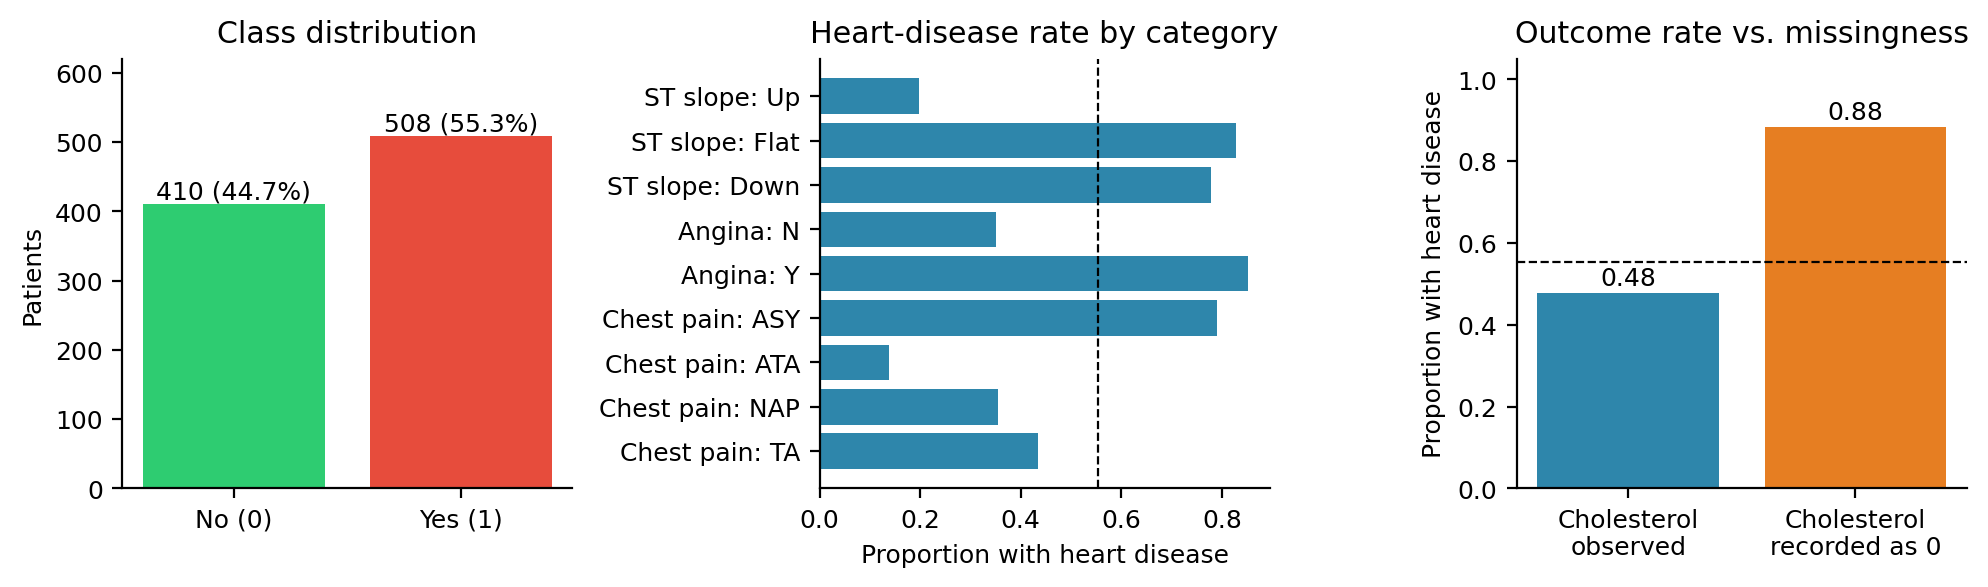
\includegraphics[width=\textwidth]{fig1_eda.png}
\caption{Class balance, heart-disease rate by selected categories (dashed line = overall 55.3\%), and outcome rate by cholesterol missingness.}\label{fig:eda}\end{figure}

\subsubsection{Tuning and cross-validated comparison}
Figure~\ref{fig:tune} shows the tuning curves. Logistic regression is flat for $C\gtrsim 0.1$ (weak regularization is enough); KNN improves up to roughly $k\approx 15$--$21$ and then plateaus; the tree benefits from a leaf-size constraint (depth 5 with at least 20 observations per leaf wins), i.e.\ from being pruned. Best CV AUC values were 0.918 (logistic regression), 0.907 (tree) and 0.910 (KNN).
\begin{figure}[H]\centering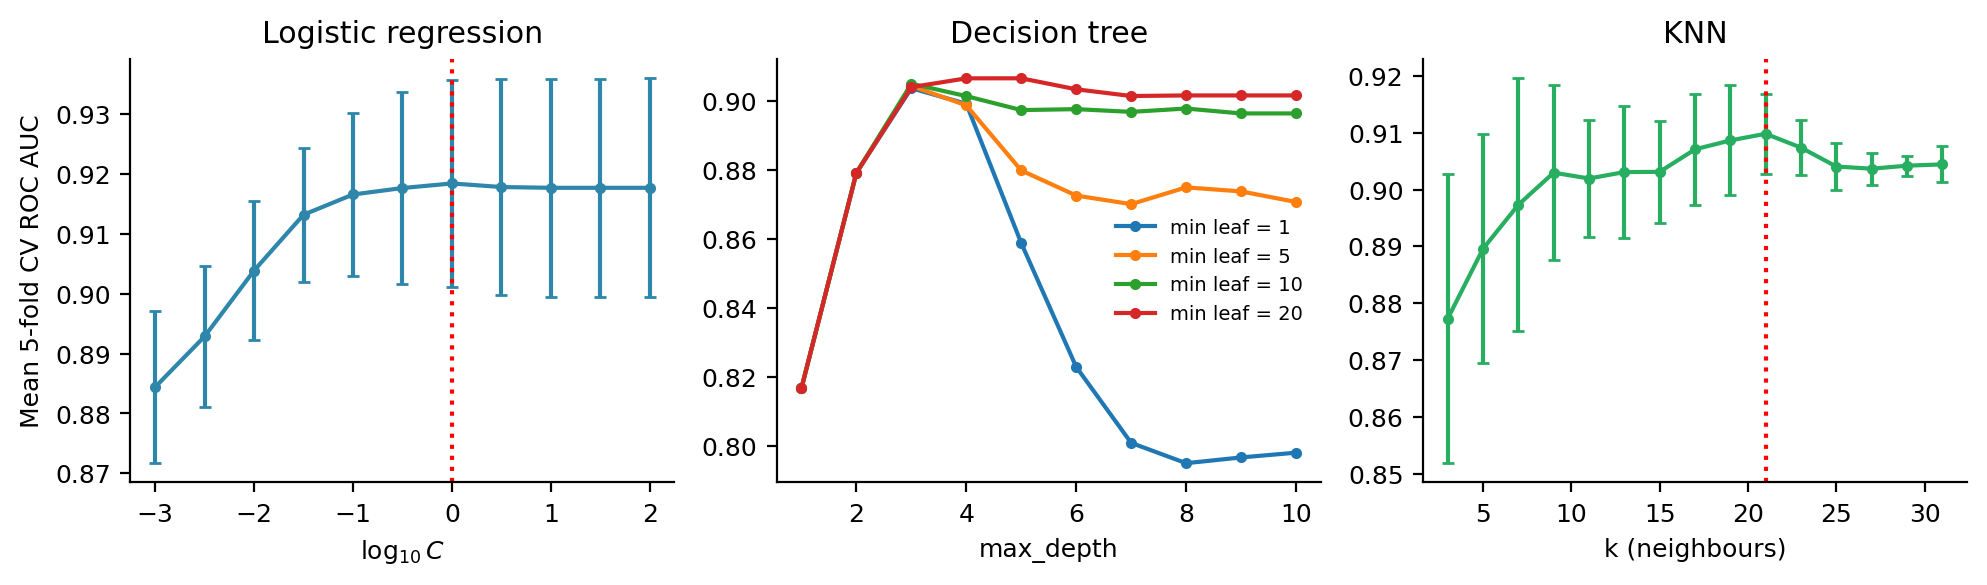
\includegraphics[width=\textwidth]{fig2_tuning.png}
\caption{Mean 5-fold CV ROC AUC on the training set over each model's grid (error bars $\pm$1 SD for LR and KNN; red dotted line = selected value).}\label{fig:tune}\end{figure}

Table~\ref{tab:nested} and Figure~\ref{fig:nested} give the nested-CV comparison, the unbiased training-side estimate. The baseline attains an F1 of 0.713 only because it labels everyone positive; its specificity is $0$ and AUC exactly $0.5$.
\begin{table}[H]\centering\small
\caption{Nested 5$\times$5 cross-validation on the training set (mean $\pm$ SD over outer folds).}\label{tab:nested}
\begin{tabular}{@{}lcccccc@{}}\toprule
Model & Accuracy & Precision & Recall & Specificity & F1 & ROC AUC\\\midrule
Majority baseline & .554$\pm$.003 & .554$\pm$.003 & 1.000 & .000 & .713$\pm$.003 & .500\\
Logistic regression & .850$\pm$.016 & .859$\pm$.033 & .877$\pm$.050 & .817$\pm$.054 & .866$\pm$.017 & .918$\pm$.016\\
Decision tree & .834$\pm$.003 & .831$\pm$.026 & .882$\pm$.044 & .775$\pm$.050 & .855$\pm$.008 & .904$\pm$.015\\
KNN & .847$\pm$.020 & .847$\pm$.018 & .884$\pm$.049 & .801$\pm$.034 & .865$\pm$.022 & .912$\pm$.012\\\bottomrule
\end{tabular}
\end{table}
\begin{figure}[H]\centering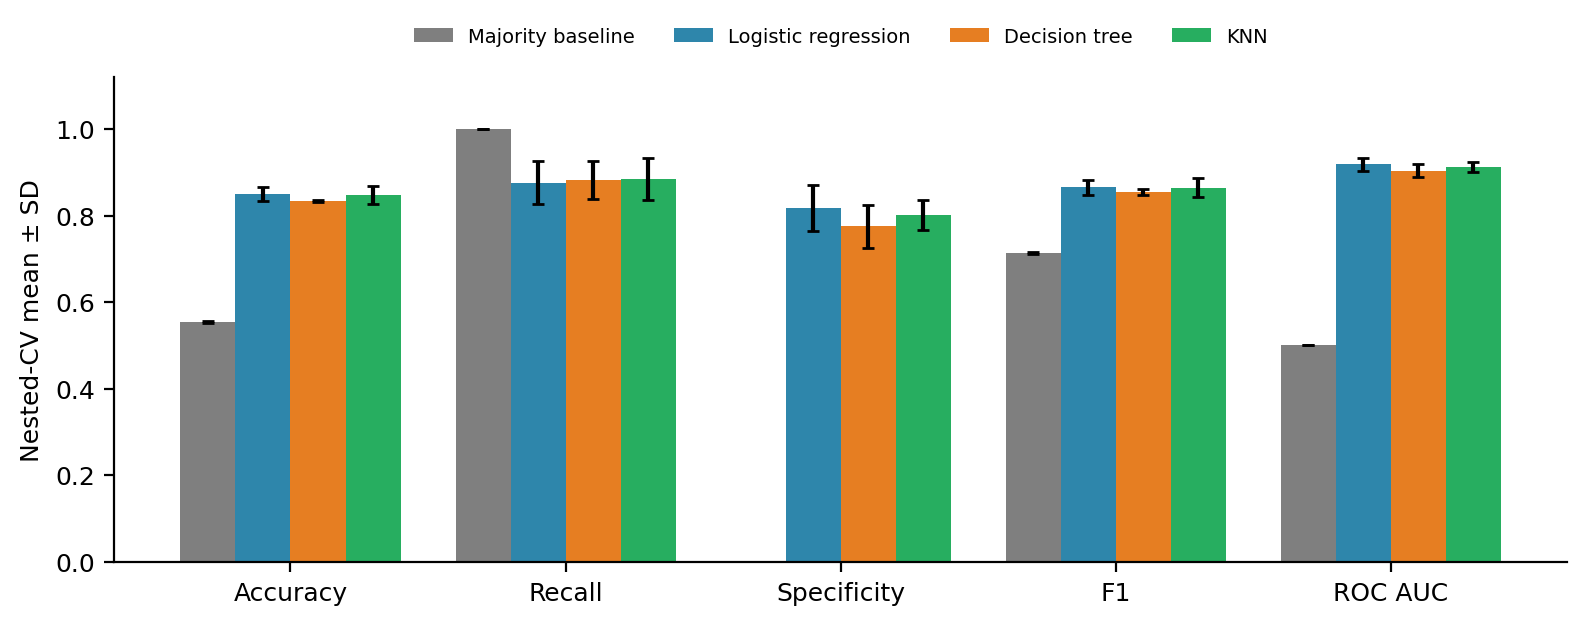
\includegraphics[width=0.85\textwidth]{fig3_nested_cv.png}
\caption{Nested-CV performance by model (mean $\pm$ SD over 5 outer folds).}\label{fig:nested}\end{figure}

\subsubsection{Held-out test performance}
Table~\ref{tab:test} reports the single test-set evaluation at the default threshold, Figure~\ref{fig:cm} the confusion matrices and Figure~\ref{fig:roc} the ROC and PR curves.
\begin{table}[H]\centering\small
\caption{Test-set performance ($n=230$; 127 positive, 103 negative) at $t=0.50$. Brackets: 95\% bootstrap CI.}\label{tab:test}
\resizebox{\textwidth}{!}{\begin{tabular}{@{}lccccccccc@{}}\toprule
Model & Acc. & Prec. & Recall & Spec. & F1 & Bal.\ acc. & MCC & ROC AUC & PR AUC\\\midrule
Majority baseline & .552 & .552 & 1.000 & .000 & .712 & .500 & .000 & .500 & .552\\
Logistic regression & \textbf{.887} & .892 & \textbf{.906} & .864 & \textbf{.898} & \textbf{.885} & \textbf{.771} & .933 & \textbf{.945}\\
Decision tree & .843 & .876 & .835 & .854 & .855 & .845 & .686 & .908 & .894\\
KNN & .883 & \textbf{.910} & .874 & \textbf{.893} & .892 & .884 & .764 & \textbf{.939} & .934\\\midrule
\multicolumn{10}{@{}l}{\emph{95\% bootstrap CIs}}\\
Logistic regression & \multicolumn{1}{c}{[.843, .926]} & & [.850, .955] & [.796, .931] & [.855, .937] & & & [.900, .964] & \\
Decision tree & [.796, .887] & & [.767, .897] & [.786, .919] & [.803, .899] & & & [.866, .946] & \\
KNN & [.839, .922] & & [.812, .929] & [.829, .952] & [.846, .929] & & & [.903, .968] & \\\bottomrule
\end{tabular}}
\end{table}
\begin{figure}[H]\centering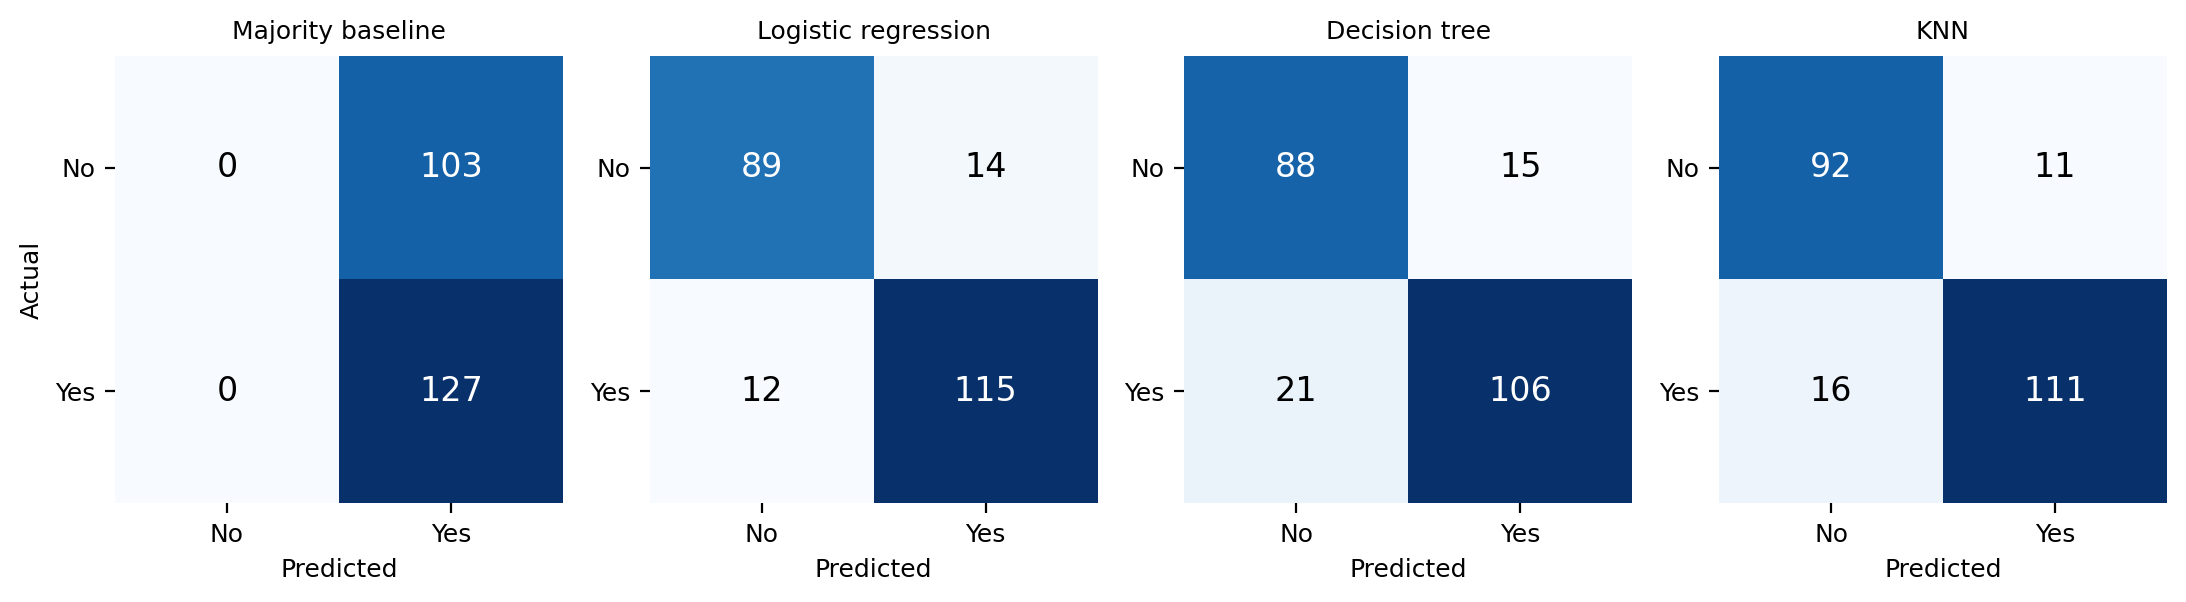
\includegraphics[width=\textwidth]{fig4_confusion.png}
\caption{Test-set confusion matrices at $t=0.50$.}\label{fig:cm}\end{figure}
\begin{figure}[H]\centering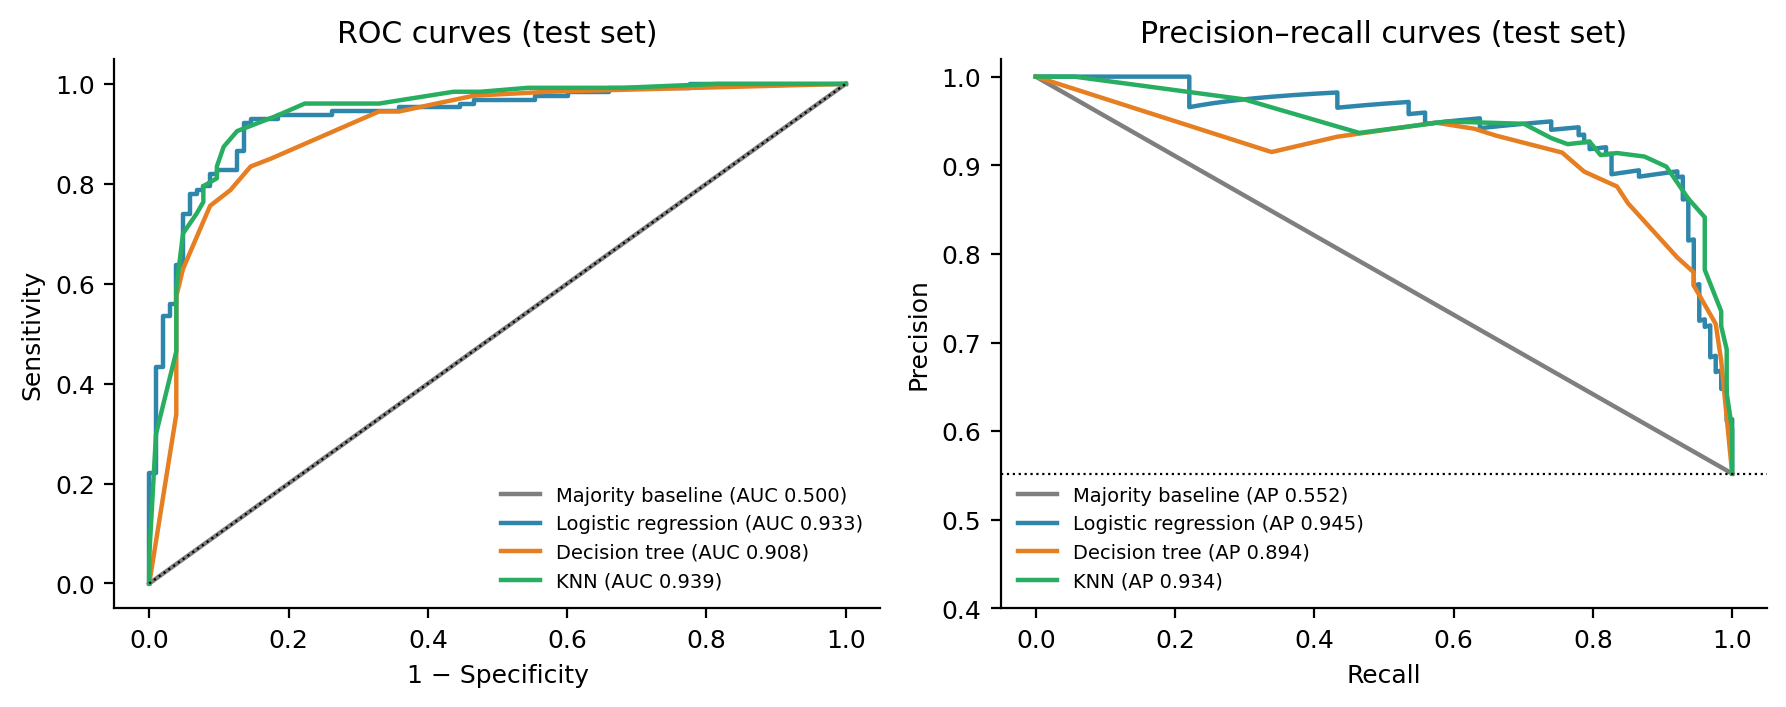
\includegraphics[width=\textwidth]{fig5_roc_pr.png}
\caption{Test-set ROC (left) and precision--recall (right) curves. The dotted PR line is the 55.2\% prevalence.}\label{fig:roc}\end{figure}

\paragraph{Significance tests.} Against the baseline, every model's exact McNemar test gives $p<10^{-10}$. Among the real models: logistic regression vs.\ tree, 17 vs.\ 7 cases uniquely correct, $p=0.064$; logistic regression vs.\ KNN, 8 vs.\ 7, $p=1.00$; KNN vs.\ tree, 15 vs.\ 6, $p=0.078$. Paired bootstrap differences in ROC AUC were $+0.025$ [0.004, 0.048] for logistic regression minus tree, $+0.031$ [0.009, 0.053] for KNN minus tree, and $-0.005$ [$-0.026$, 0.016] for logistic regression minus KNN.

\subsubsection{Interpretability}
Figure~\ref{fig:interp} shows what the two transparent models learned. Both rank the same signals highest: ST-slope shape, asymptomatic chest pain, exercise angina and maximum heart rate. In logistic regression, the largest positive coefficients are asymptomatic chest pain ($+1.30$), male sex ($+1.27$), fasting blood sugar $>120$ mg/dL ($+1.25$) and a flat ST slope ($+1.02$); an upward ST slope is the largest protective effect ($-1.22$). Male sex, high fasting sugar and ASY pain each correspond to roughly 3.5--3.7 times higher odds, other things equal. The tree's root split is \code{ST\_Slope\_Up} (importance 0.68), followed by asymptomatic chest pain (0.16) and \code{MaxHR} (0.07); the tree has depth 5 and 16 leaves (Figure~\ref{fig:tree}). \code{Cholesterol} contributes little in either model (coefficient $+0.05$, tree importance 0.009).
\begin{figure}[H]\centering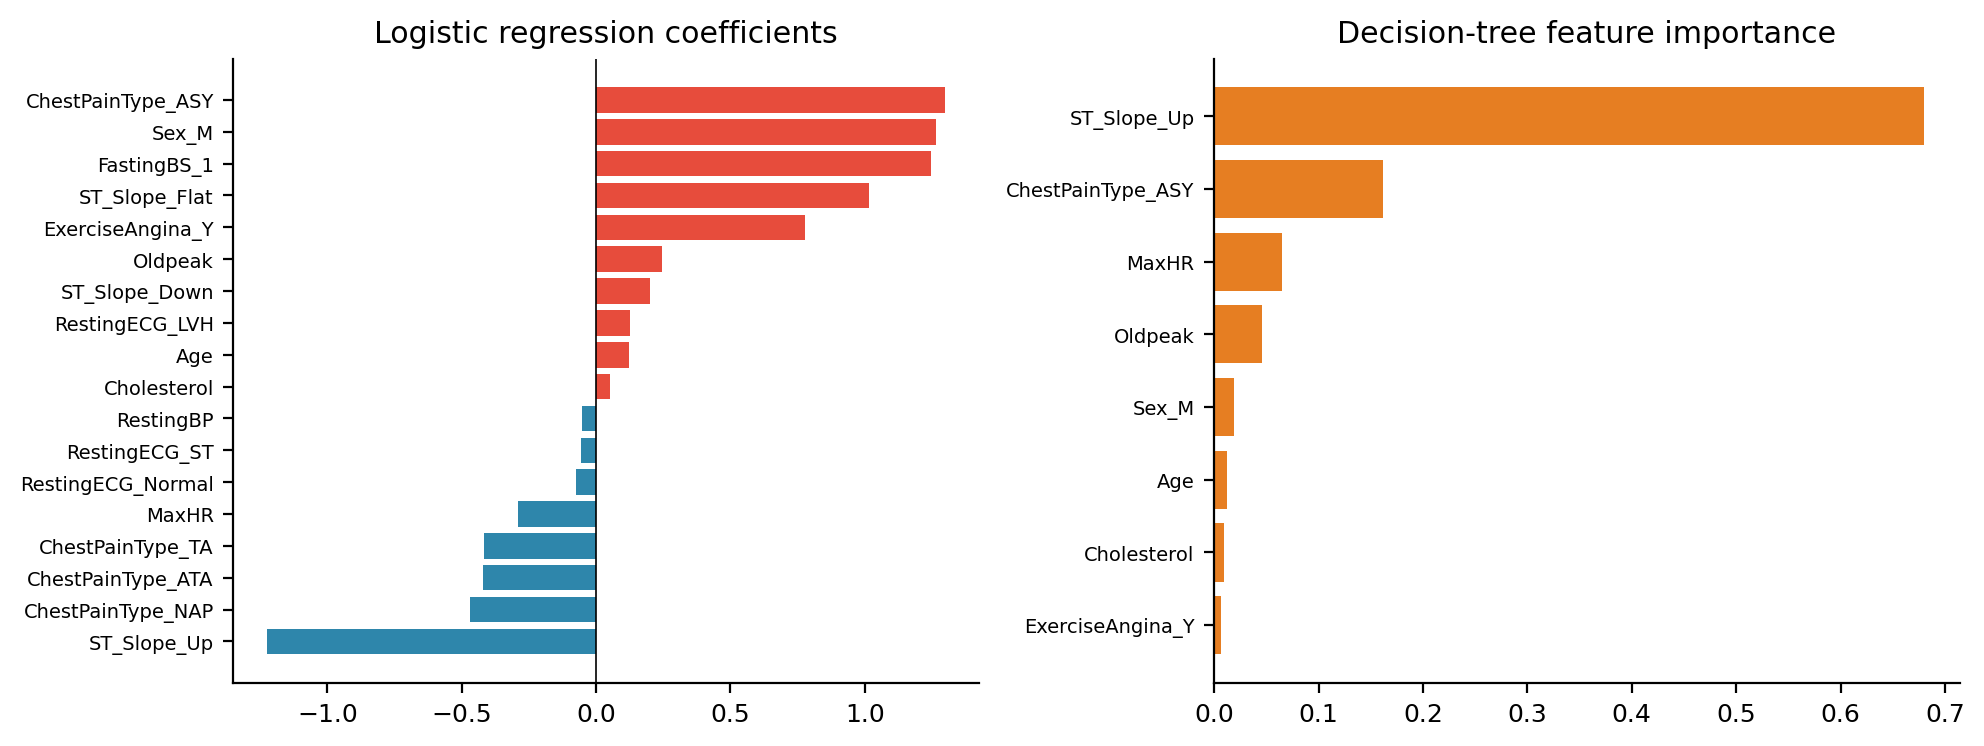
\includegraphics[width=\textwidth]{fig6_interpretability.png}
\caption{Logistic-regression coefficients (numeric features standardized; red = raises risk) and decision-tree feature importances.}\label{fig:interp}\end{figure}
\begin{figure}[H]\centering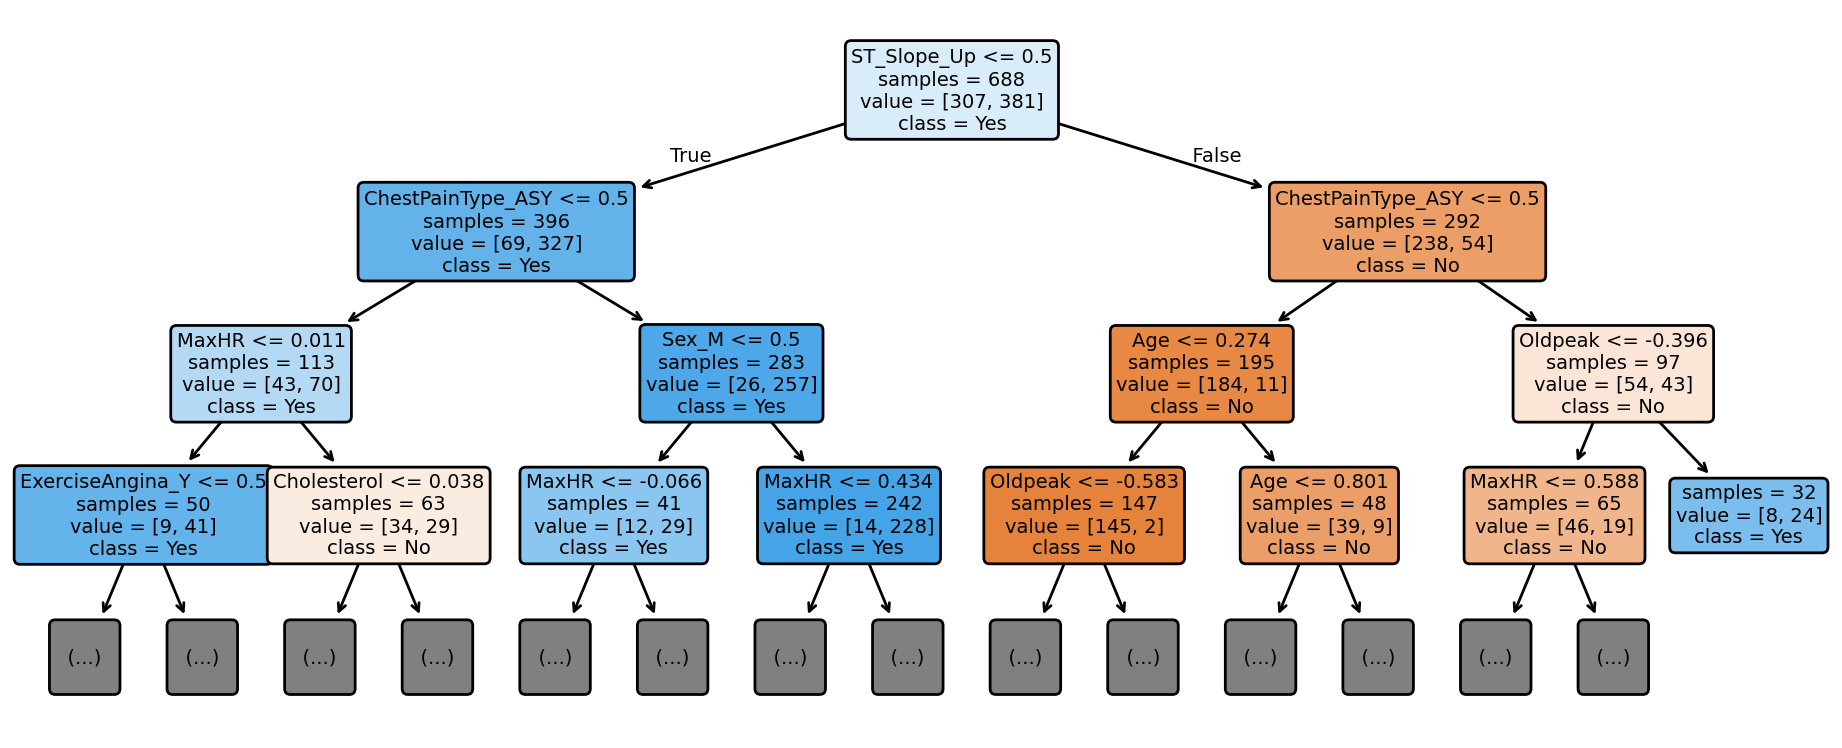
\includegraphics[width=\textwidth]{fig7_tree.png}
\caption{Top three levels of the selected decision tree. Numeric thresholds are on the standardized scale (z-scores); \code{value} = [negative, positive] training counts.}\label{fig:tree}\end{figure}

\subsubsection{Cost-sensitive threshold}\label{sec:cost}
Suppose a missed patient costs $5$ units and a false alarm $1$ (an assumption for illustration, not an estimated clinical cost). Using out-of-fold training predictions, the cost-minimizing thresholds were $0.22$ (logistic regression), $0.22$ (tree) and $0.32$ (KNN), somewhat above the theoretical $1/6\approx 0.17$; the gap reflects imperfectly calibrated probabilities and the coarse threshold grid. Table~\ref{tab:cost} applies them to the test set; Figure~\ref{fig:cost} shows the training-side cost curves.
\begin{table}[H]\centering\small
\caption{Test-set errors and expected cost ($5\cdot FN+1\cdot FP$) at the default and cost-tuned thresholds.}\label{tab:cost}
\begin{tabular}{@{}lccccccccc@{}}\toprule
 & \multicolumn{4}{c}{Default $t=0.50$} & & \multicolumn{4}{c}{Tuned $t^\ast$ (from OOF)}\\\cmidrule{2-5}\cmidrule{7-10}
Model & FN & FP & Cost & & $t^\ast$ & FN & FP & Cost\\\midrule
Majority baseline & 0 & 103 & 103 & & --- & --- & --- & ---\\
Logistic regression & 12 & 14 & 74 & & 0.22 & 7 & 32 & 67\\
Decision tree & 21 & 15 & 120 & & 0.22 & 7 & 34 & 69\\
KNN & 16 & 11 & 91 & & 0.32 & 5 & 29 & \textbf{54}\\\bottomrule
\end{tabular}
\end{table}
\begin{figure}[H]\centering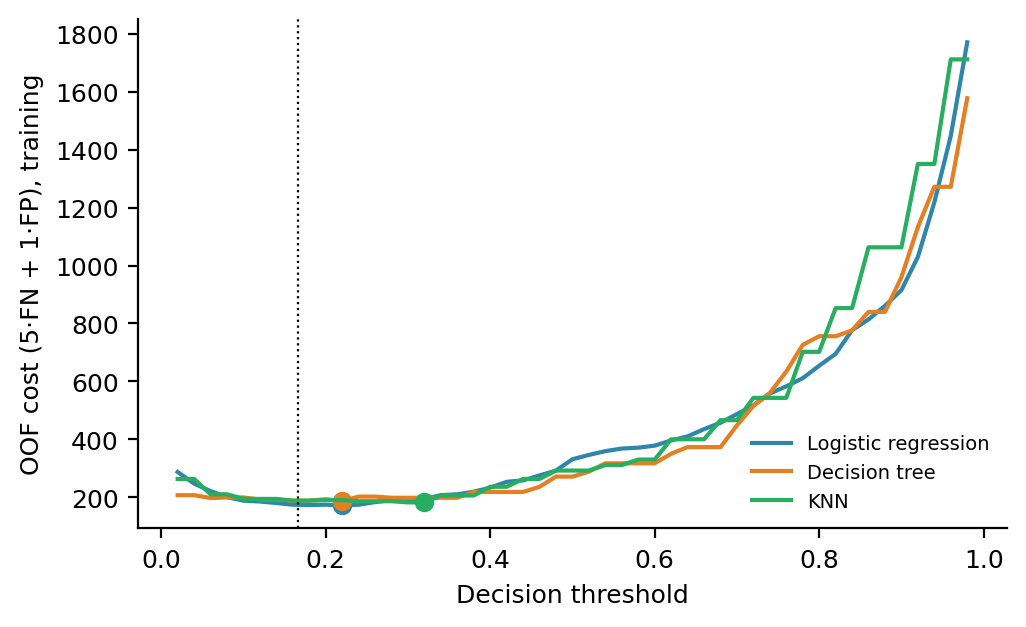
\includegraphics[width=0.55\textwidth]{fig8_cost.png}
\caption{Out-of-fold cost versus threshold on the training set (dots = chosen thresholds; dotted line = $1/6$).}\label{fig:cost}\end{figure}

\subsection{Analysis and Discussion}
\paragraph{The baseline shows why metric choice matters.} Because the majority class is positive, the baseline has the \emph{highest recall} (1.00) and a respectable F1 (0.712) while being useless: it flags all 103 healthy test patients. Only specificity, balanced accuracy, MCC and ROC AUC expose this (0.00, 0.50, 0.00, 0.50). Reading accuracy or F1 alone would understate how much the models add, and reading recall alone would reward the baseline.

\paragraph{All models learn real signal.} Relative to the baseline, test accuracy rises by 29--34 percentage points and MCC from 0 to 0.69--0.77. The McNemar results leave no doubt that this is not chance.

\paragraph{Logistic regression $\approx$ KNN $>$ tree.} In both nested CV and the test set, logistic regression and KNN are practically tied (AUC difference $-0.005$, CI containing 0; McNemar $p=1.0$), and each is about 0.025--0.03 AUC above the tree, a difference whose bootstrap CI excludes zero for AUC but whose McNemar tests on accuracy are borderline ($p=0.064$, $0.078$). With 230 test patients the CIs are wide ($\approx\pm$4 points for accuracy), so we read the ordering as ``tree somewhat worse'' rather than as a precise ranking of the top two. A likely reason for the tree's deficit is its coarse score: with 16 leaves it outputs only 16 distinct probabilities, which degrades ranking (AUC), and axis-aligned splits approximate a smooth risk gradient less well than a linear score. That the near-linear model is as accurate as flexible KNN suggests that the class boundary in these predictors is well approximated by a roughly linear log-odds surface.

\paragraph{Different error profiles.} At $t=0.5$ KNN is the most specific (0.893) and precise (0.910) but misses 16 patients; logistic regression is the most sensitive (0.906) with 12 misses; the tree misses the most (21). Which is preferable depends on the relative cost of errors, which is why the threshold analysis matters: after cost tuning, all three models reduced cost below the baseline's 103, with KNN lowest (54) and logistic regression at 67. The cost ordering at tuned thresholds (KNN $<$ LR) differs from the AUC ordering by a small margin that may reflect test-set noise, since a single threshold on 230 patients is a noisy quantity; the cost-tuned recall of 0.94--0.96 comes at specificity of 0.67--0.72.

\paragraph{Computational cost.} All four models train and predict in milliseconds on 688 rows, so cost does not separate them at this scale. Structurally, logistic regression compresses the data into 18 coefficients, whereas KNN must store the whole training set and compute distances at prediction time, which scales poorly with data size; the tree's grid search was the slowest only because its grid is the largest.

\paragraph{Missing cholesterol.} Because zero-cholesterol rows are $88\%$ positive, a ``missing'' indicator is potentially informative. Adding one raised nested-CV AUC slightly for logistic regression (0.918 to 0.928) and KNN (0.912 to 0.918) and lowered it for the tree (0.904 to 0.900), all within one fold SD. We did not adopt it in the main pipeline because it exploits a data-collection artifact (which source hospital recorded cholesterol) rather than physiology, and it would likely not transfer to a hospital with complete records.

\paragraph{Limitations and assumptions.}
\begin{itemize}[leftmargin=2em,itemsep=0pt]
\item \textbf{Small, single split.} The test set has 230 patients; metric CIs are $\approx\pm$4--8 points and nested CV SDs are 1--5 points, so small differences between the top models are not reliable.
\item \textbf{Pooled sources.} Five collections with different protocols were merged and there is no hospital identifier, so we cannot test cross-site generalization; the cholesterol artifact above is one symptom.
\item \textbf{Zero-as-missing assumption} (A1) and median imputation may blur true variation; imputation of 18.7\% of one feature is substantial.
\item \textbf{Assumed costs.} The $5{:}1$ ratio is illustrative; probabilities from trees and KNN are not calibrated, so thresholds are heuristic.
\item \textbf{Limited tuning.} Only one or two hyperparameters per model were tuned; other models (e.g.\ ensembles) were out of scope.
\item \textbf{Not a clinical validation.} These are retrospective records; no prospective or external validation was done.
\end{itemize}

\section{Conclusion}
On 918 patient records, logistic regression, a pruned decision tree and KNN all substantially outperformed a majority-class baseline, which despite 100\% recall and an F1 of 0.71 had no discriminating ability (specificity 0, MCC 0, AUC 0.5). Logistic regression ($C=1$) and KNN ($k=21$) were the strongest and statistically indistinguishable (test accuracy 0.887 vs.\ 0.883, AUC 0.933 vs.\ 0.939); the tree (depth 5) was about 4 points less accurate but yielded readable rules that agree with the logistic coefficients on the key predictors (ST slope, chest-pain type, exercise angina, maximum heart rate). Because KNN offers no accuracy advantage over logistic regression while requiring the stored training set and offering no coefficients, we recommend \textbf{logistic regression as the default screening model}, keeping the tree as an explanation aid. Lowering the threshold using out-of-fold predictions reduced the illustrative 5:1 cost for every model.

\section{Recommendations and Future Directions}
Based on the findings, we recommend logistic regression as the default screening model and retaining the decision tree as an explanation aid. Possible extensions follow.
 (1) Repeated or grouped cross-validation, and external validation on local patient data; (2) probability calibration (Platt scaling or isotonic regression) before choosing thresholds; (3) estimating real clinical costs rather than assuming them; (4) feature-selection and ensemble methods such as random forests and gradient boosting; (5) a missing-data model that does not rely on collection artifacts; and (6) a prospective pilot in advisory mode with clinician review.

\newpage
\begin{thebibliography}{99}
\setlength{\itemsep}{0.6em}

\bibitem{r0}
Avendano, B. F. B., De Robles, L. C. C., Ignacio, C. W. B., Manlapig, J. L. V., \& Robles, B. J. G. (2026). \emph{Heart failure prediction using K-nearest neighbors} [Unpublished course report]. Bulacan State University.

\bibitem{r1}
Breiman, L., Friedman, J. H., Olshen, R. A., \& Stone, C. J. (1984). \emph{Classification and regression trees}. Wadsworth.

\bibitem{r2}
Chicco, D., \& Jurman, G. (2020). The advantages of the Matthews correlation coefficient (MCC) over F1 score and accuracy in binary classification evaluation. \emph{BMC Genomics, 21}, Article 6. https://doi.org/10.1186/s12864-019-6413-7

\bibitem{r3}
Cover, T., \& Hart, P. (1967). Nearest neighbor pattern classification. \emph{IEEE Transactions on Information Theory, 13}(1), 21--27. https://doi.org/10.1109/TIT.1967.1053964

\bibitem{r5}
Detrano, R., Janosi, A., Steinbrunn, W., Pfisterer, M., Schmid, J.-J., Sandhu, S., Guppy, K. H., Lee, S., \& Froelicher, V. (1989). International application of a new probability algorithm for the diagnosis of coronary artery disease. \textit{The American Journal of Cardiology, 64}(5), 304--310. https://doi.org/10.1016/0002-9149(89)90524-9

\bibitem{r4}
Dietterich, T. G. (1998). Approximate statistical tests for comparing supervised classification learning algorithms. \emph{Neural Computation, 10}(7), 1895--1923. https://doi.org/10.1162/089976698300017197

\bibitem{rx}
Efron, B. (1979). Bootstrap methods: Another look at the jackknife. \emph{The Annals of Statistics, 7}(1), 1--26. https://doi.org/10.1214/aos/1176344552

\bibitem{r6}
Elkan, C. (2001). The foundations of cost-sensitive learning. In \emph{Proceedings of the 17th International Joint Conference on Artificial Intelligence} (pp. 973--978). Morgan Kaufmann.

\bibitem{r7}
Fawcett, T. (2006). An introduction to ROC analysis. \emph{Pattern Recognition Letters, 27}(8), 861--874. https://doi.org/10.1016/j.patrec.2005.10.010

\bibitem{r8}
Fedesoriano. (2021). \emph{Heart failure prediction dataset} [Data set]. Kaggle. https://www.kaggle.com/datasets/fedesoriano/heart-failure-prediction

\bibitem{r9}
Hosmer, D. W., Lemeshow, S., \& Sturdivant, R. X. (2013). \emph{Applied logistic regression} (3rd ed.). Wiley.

\bibitem{r10}
Pedregosa, F., Varoquaux, G., Gramfort, A., Michel, V., Thirion, B., Grisel, O., Blondel, M., Prettenhofer, P., Weiss, R., Dubourg, V., Vanderplas, J., Passos, A., Cournapeau, D., Brucher, M., Perrot, M., \& Duchesnay, {\'E}. (2011). Scikit-learn: Machine learning in Python. \emph{Journal of Machine Learning Research, 12}, 2825--2830.

\bibitem{r11}
Saito, T., \& Rehmsmeier, M. (2015). The precision-recall plot is more informative than the ROC plot when evaluating binary classifiers on imbalanced datasets. \emph{PLOS ONE, 10}(3), Article e0118432. https://doi.org/10.1371/journal.pone.0118432

\bibitem{r12}
Varma, S., \& Simon, R. (2006). Bias in error estimation when using cross-validation for model selection. \emph{BMC Bioinformatics, 7}, Article 91. https://doi.org/10.1186/1471-2105-7-91

\bibitem{r13}
World Health Organization. (2025). \emph{Cardiovascular diseases (CVDs)}. https://www.who.int/news-room/fact-sheets/detail/cardiovascular-diseases-(cvds)

\end{thebibliography}

\newpage
%================ APPENDIX ================
\appendix
\section{Reproducibility and Code Repository}
The Git repository contains: \code{data/heart.csv}; \code{src/analysis.py} (complete pipeline, tuning, nested CV, tests, figures); \code{results/} (\code{results.json}, \code{test\_metrics.csv}, \code{nested\_cv.csv}, \code{tree\_rules.txt}); \code{figures/}; \code{paper/main.tex}; \code{requirements.txt}; and a \code{README.md}. Run \code{pip install -r requirements.txt} then \code{python src/analysis.py}. A global seed of 42 fixes the split, fold assignment and tree construction; scikit-learn 1.8.0 was used.

\end{document}
